\documentclass[tikz]{standalone}
\usepackage{tikz}
\usepackage{amssymb}
\usetikzlibrary{positioning}
\usetikzlibrary{calc}
\usetikzlibrary{arrows,shapes,snakes,automata,petri}
\begin{document}
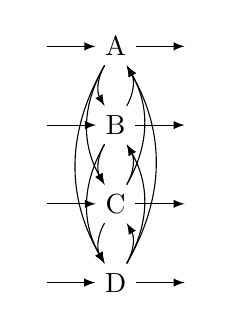
\begin{tikzpicture}
\node[](startA) at (-1,0){};
\node[](startB) at (-1,-1){};
\node[](startC) at (-1,-2){};
\node[](startD) at (-1,-3){};
\node[](A) at (0,0){A};
\node[](B) at (0,-1){B};
\node[](C) at (0,-2){C};
\node[](D) at (0,-3){D};
\node[](endA) at (1,0){};
\node[](endB) at (1,-1){};
\node[](endC) at (1,-2){};
\node[](endD) at (1,-3){};

\path
(startA) edge[-latex]node{} (A)
(startB) edge[-latex]node{} (B)
(startC) edge[-latex]node{} (C)
(startD) edge[-latex]node{} (D)
(A) edge[-latex,bend right]node{} (B)
(A) edge[-latex,bend right]node{} (C)
(A) edge[-latex,bend right]node{} (D)
(B) edge[-latex,bend right]node{} (A)
(B) edge[-latex,bend right]node{} (C)
(B) edge[-latex,bend right]node{} (D)
(C) edge[-latex,bend right]node{} (A)
(C) edge[-latex,bend right]node{} (B)
(C) edge[-latex,bend right]node{} (D)
(D) edge[-latex,bend right]node{} (A)
(D) edge[-latex,bend right]node{} (B)
(D) edge[-latex,bend right]node{} (C)
(A) edge[-latex]node{} (endA)
(B) edge[-latex]node{} (endB)
(C) edge[-latex]node{} (endC)
(D) edge[-latex]node{} (endD);
\end{tikzpicture}
\end{document}